%\hyphenation{Волоколамский}
\documentclass[14pt,a4paper,twoside]{article} 

\pdfgentounicode=1
\sloppy

\newcommand*{\No}{\textnumero} %R_2

\newcommand{\issueYear}{0000}
\newcommand{\issueVolume}{0}
\newcommand{\issueMnthsRu}{Месяц -- Месяц 0 (00)}
\newcommand{\issueMnthsEn}{Month -- Month 0 (00)}

\usepackage[T1,T2A]{fontenc}
\usepackage[utf8]{inputenc}
\usepackage[english,russian]{babel}
\usepackage{amsmath,amsfonts,amssymb,amscd,euscript}
\usepackage{mathrsfs}
\usepackage{epsfig,epstopdf}
\usepackage{manyfoot}

\oddsidemargin=0mm 
\evensidemargin=2mm 
\textheight=690pt 
\topmargin=-14mm
\textwidth=450pt 
%\headsep=10mm
\headheight=14pt
\setlength\parindent{5ex}

\usepackage{anyfontsize}

\usepackage[%
	pdfpagemode=UseNone,%
    pdfpagelayout=TwoPageLeft,%
    bookmarks=false,%
    bookmarksopenlevel=1,%
	breaklinks,%
	draft%
]{hyperref}        
\usepackage[all]{hypcap}
\usepackage{cite}


%%%%%%%%%%%%%%%%%%%%%%
\addto\captionsrussian{%
  \renewcommand{\UDKName}{УДК}%  
  \renewcommand{\AbstractWords}{Аннотация}% 
  \renewcommand{\KeyWords}{Ключевые слова}%
  \renewcommand{\contentsname}{СОДЕРЖАНИЕ}%
  \renewcommand{\indexname}{АВТОРСКИЙ УКАЗАТЕЛЬ}%
  \renewcommand\refname{\normalsize Список литературы}%
  \renewcommand\receivedWords{Поступила  в редакцию}%
  \renewcommand{\figurename}{Рис.}%
  \renewcommand{\citeString}{
    \textbf{Просьба ссылаться на эту статью следующим образом:}\\
    {\the\authorslistInv} {\csname title\endcsname}. {\it Вестник МГТУ МИРЭА 2015 №1 (6)}. \issueYear. №~\issueVolume. \mbox{C.~\pageref{\theArticle:article:fstpage}–-\pageref{\theArticle:article:lastpage}}.
  }%
  \renewcommand{\issueMnths}{\issueMnthsRu}%
}
\addto\captionsenglish{%
  \renewcommand{\UDKName}{UDC}%   
  \renewcommand{\AbstractWords}{Abstract}% 
  \renewcommand{\KeyWords}{Keywords}%
  \renewcommand{\contentsname}{CONTENTS}%
  \renewcommand{\indexname}{INDEX OF AUTHORS}%
  \renewcommand\refname{\normalsize References}%
  \renewcommand\receivedWords{Received}%
  \renewcommand{\figurename}{Fig.}%
  \renewcommand{\citeString}{
    \textbf{Please cite this article in English as:}\\
    {\the\authorslistInvSub} {\csname titleSub\endcsname}. {\it Space, Time and Fundamental Interactions}, \issueYear, no.~\issueVolume, \mbox{pp.~\pageref{\theArticle:article:fstpage}--\pageref{\theArticle:article:lastpage}}.
  }%
  \renewcommand{\issueMnths}{\issueMnthsEn}%
}

%
\addto\extrasrussian{\renewcommand\figureautorefname{Рис.}}
\addto\extrasenglish{\renewcommand\figureautorefname{Fig.}}

\renewcommand{\tiny}{\fontsize{5}{8}\selectfont}
\renewcommand{\scriptsize}{\fontsize{7}{10}\selectfont}
\renewcommand{\footnotesize}{\fontsize{8}{10}\selectfont}
\renewcommand{\small}{\fontsize{9}{12}\selectfont}
\renewcommand{\normalsize}{\fontsize{10}{14}\selectfont}
\renewcommand{\large}{\fontsize{11}{16}\selectfont}
\renewcommand{\Large}{\fontsize{12}{18}\selectfont}
\renewcommand{\LARGE}{\fontsize{14}{21}\selectfont}
\renewcommand{\huge}{\fontsize{16}{24}\selectfont}
\renewcommand{\Huge}{\fontsize{20}{30}\selectfont}
%
\usepackage[scaled=1.2]{PTSansNarrow}
\usepackage[scaled=.9]{PTMono}
%
\newcounter{Article}
\renewcommand{\theArticle}{\arabic{Article}}
%\renewcommand\theequation{\arabic{equation}}
\numberwithin{equation}{section}
\renewcommand{\theequation}{\arabic{section}.\arabic{equation}}

\usepackage{xstring}

%%%%%%%%%%%%%%%%%%%%%%%%%%%%%%%%%%%%%%%%%%%%%%%%%%%%%%%%%%%%%%%%%%%%%%%%%%%%%%%

\usepackage[explicit]{titlesec}

\titleformat{\section}%
  {\normalfont\bfseries}%
  {}%
  {0em}%
  {\normalfont\bfseries\textbf{\thesection.\hspace{0.02em} #1}}% в другом  \hspace{0.02em} #1}}
  
\titleformat{name=\section,numberless}%
  {\normalfont\bfseries}%
  {}%
  {0em}%
  {\normalfont\bfseries #1}%\MakeUppercase{#1}}

\titlespacing*{\section}{0pt}{1em}{1em}

\titleformat{\subsection}%
  {\normalfont\itshape\bfseries}%
  {}%
  {0em}%
  %{\normalfont\itshape\bfseries\thesubsection.\hspace{1em} #1}
	{\normalfont\bfseries\thesubsection.\hspace{0.2em} #1}
  
\titleformat{name=\subsection,numberless}%
  {\normalfont\itshape}%
  {}%
  {0em}%
  {\normalfont\itshape #1}

\titlespacing*{\subsection}{0pt}{1em}{1em}

\renewcommand*\thesection{\arabic{section}}


\newcommand{\DOIM}{DOI: 10.17238/issn2226-8812.2018.2}

%%%%%%%%%%%%%%%%%%%%%%%%%%%%%%%%%%%%%%%%%%%%%%%%%%%%%%%%%%%%%%%%%%%%%%%%%%%%%%%
%
% images
%
\usepackage{caption}
\DeclareCaptionFont{white}{\color{white}}
\DeclareCaptionFormat{overlay}{\small{\bfseries #1.}{\hskip 1em}#3}
\DeclareCaptionFormat{empty}{}
\captionsetup{format=overlay,font={},labelfont={bf}}
%\renewcommand\thefigure{\arabic{figure}}
%
%%%%%%%%%%%%%%%%%%%%%%%%%%%%%%%%%%%%%%%%%%%%%%%%%%%%%%%%%%%%%%%%%%%%%%%%%%%%%%%
%
% колонтитулы
%
\usepackage{fancyhdr}
\fancypagestyle{firstpage}
{
  \fancyhf{}
  \renewcommand{\headrulewidth}{1pt}
  \renewcommand{\footrulewidth}{0pt}

	\fancyhead[LE,LO]{\footnotesize Вестник МГТУ МИРЭА 2015 № 1 (6)}
}

\fancypagestyle{firstpage_arxiv}
{
  \fancyhf{}
  \renewcommand{\headrulewidth}{1pt}
  \renewcommand{\footrulewidth}{0pt}

	\fancyhead[LE,LO]{\footnotesize Herald of MSTU MIREA 2015 № 1 (6)}
  \fancyhead[RE,RO]{\footnotesize \issueYear, vol. \issueVolume}
}

\fancypagestyle{outputpage}{
  \fancyhf{}
  \renewcommand{\headrulewidth}{0pt}
  \renewcommand{\footrulewidth}{0pt}
  \fancyhead[LE,LO]{\DOIM}
  \fancyhead[RE,RO]{\issueMnths\quad \issueYear}
}
% http://tex.stackexchange.com/questions/59468/how-to-cut-chapter-title-in-header-using-xstring?rq=1  
%\renewcommand{\sectionmark}[1]{\markright{\thesection\ \protect\StrLeft{#1}{65}}{}}
%
\fancypagestyle{commonpage}{
  \fancyhf{}
  \renewcommand{\headrulewidth}{1pt}
  \renewcommand{\footrulewidth}{0pt}
  \fancyhead[LE,RO]{\normalsize\thepage}
  \fancyhead[LO]{\footnotesize\rightmark}
  \fancyhead[RE]{\footnotesize\leftmark}
}
\pagestyle{commonpage}

\renewcommand{\sectionmark}[1]{}
\renewcommand{\subsectionmark}[1]{}
%
%%%%%%%%%%%%%%%%%%%%%%%%%%%%%%%%%%%%%%%%%%%%%%%%%%%%%%%%%%%%%%%%%%%%%%%%%%%%%%%
%
% Automatically typeset math in section headings in bold-face
% http://tex.stackexchange.com/questions/41379/automatically-typeset-math-in-section-headings-in-bold-face
%
\makeatletter
\g@addto@macro\bfseries{\boldmath}
\makeatother
%
%%%%%%%%%%%%%%%%%%%%%%%%%%%%%%%%%%%%%%%%%%%%%%%%%%%%%%%%%%%%%%%%%%%%%%%%%%%%%%%
%
% firstindent
%
\makeatletter
\let\@afterindentfalse\@afterindenttrue
\makeatother


%%%%%%%%%%%%%%%%%%%%%%%%%%%%%%%%%%%%%%%%%%%%%%%%%%%%%%%%%%%%%%%%%%%%%%%%%%%%%%%
% Листинг кода
%
\usepackage{listings}
% Define Language
\lstdefinelanguage{Maple}
{
  % list of keywords
  morekeywords={
    abs,animate,array,assuming,
    Christoffel1,Christoffel2,collect,create,cov_diff,
	d1metric,d2metric,DEplot,diff,Dirac,display,do,dsolve,dual,
    Einstein,end,eval,evalf,expand,
	for,from,
	Heaviside,
	if,implicitplot,innerprod,int,interface,invert,
	geodesic_eqns,get_char,get_compts,get_rank,grad,
	Levi_Civita,lin_com,local,lhs,
	matadd,
	odeplot,op,
	piecewise,plot,plot3d,point,pointplot,proc,prod,
	Ricci,Ricciscalar,Riemann,restart,rhs,
	scalarmul,seq,signum,simplify,solve,spacecurve,sqrt,subs,sum,
	to,trunc,
	union,
	with
  },
  sensitive=false, 					% keywords are not case-sensitive
  morecomment=[l]{\#}, 				% l is for line comment
  morecomment=[s]{/*}{*/}, 			% s is for start and end delimiter
  morestring=[b]" 					% defines that strings are enclosed in double quotes
}
% Set Language
\lstset{
    extendedchars=true, 				% русские буквы в комментариях были
    basicstyle=\small\ttfamily,	% размер и начертание шрифта для подсветки кода
    %keywordstyle=\ttfamily\bfseries,	% размер и начертание шрифта для ключевых слов
    numbers=left,               		% где поставить нумерацию строк (слева\справа)
    numberstyle=\footnotesize,          % размер шрифта для номеров строк
    stepnumber=1,                   	% размер шага между двумя номерами строк
    numbersep=10pt,                		% как далеко отстоят номера строк от подсвечиваемого кода
    showspaces=false,            		% показывать или нет пробелы специальными отступами
    showstringspaces=false,      		% показывать или нет пробелы в строках
    showtabs=false,             		% показывать или нет табуляцию в строках
    frame=false,              			% не рисовать рамку вокруг кода
    tabsize=2,                 			% размер табуляции по умолчанию равен 2 пробелам
    % caption=t,              			% позиция заголовка вверху [t] или внизу [b]
    breaklines=true,           			% автоматически переносить строки (да\нет)
    breakatwhitespace=false, 			% переносить строки только если есть пробел
    morecomment=[l]{\#},				% символ начала строки коментария
    escapeinside={\%*}{*)},   			% если нужно добавить комментарии в коде
    commentstyle=\normalsize,
    stringstyle=\normalsize,
	xleftmargin=.05\textwidth,
} 

%%%%%%%%%%%%%%%%%%%%%%%%%%%%%%%%%%%%%%%%%%%%%%%%%%%%%%%%%%%%%%%%%%%%%%%%%%%%%%%
%
% VARIABLES
%%%%%%%%%%%%%%%%%%%%%%
\newtoks{\affillistRu}
\newtoks{\affillistEn}
\newtoks{\mailList}
%\newtoks{\grant}
\newtoks{\authorslist}
\newtoks{\authorslistSub}
\newtoks{\authorslistInv}
\newtoks{\authorslistInvIndex}
\newtoks{\authorslistInvIndexSub}
\newtoks{\authorslistFooter}
\newtoks{\authorslistFooterSub}
\newtoks{\authorslistInvSub}
%%
\newcount\articleslanguage
\newcount\loopingindex % NOT inside the definition!


\newcommand{\AbstractWords}{}
\newcommand{\KeyWords}{}
\newcommand{\UDKName}{}
\newcommand{\receivedWords}{}
\newcommand{\citeString}{}
\newcommand{\issueMnths}{}
\newcommand{\sourceAuthor}{}
\newlength\boxheight
%
\newcounter{numauthors}
%
% COMMANDS
%
\newcommand{\affili}[3]{
  \global\affillistRu=\expandafter{\the\affillistRu \text{$^{#1 \ }$} {#2}  \newline}
	\global\affillistEn=\expandafter{\the\affillistEn \text{$^{#1 \ }$} {#3}  \newline}
}
\newcommand{\addauthor}[1]{%
  \global\authorslist=\expandafter{\the\authorslist#1}
}
\newcommand{\addauthorSub}[1]{%
  \global\authorslistSub=\expandafter{\the\authorslistSub#1}
}
\newcommand{\addauthorInv}[1]{%
  \global\authorslistInv=\expandafter{\the\authorslistInv#1}
}
\newcommand{\addauthorInvIndex}[1]{%
  \global\authorslistInvIndex=\expandafter{\the\authorslistInvIndex#1}
}
\newcommand{\addauthorInvIndexSub}[1]{%
  \global\authorslistInvIndexSub=\expandafter{\the\authorslistInvIndexSub#1}
}
\newcommand{\addauthorFooter}[2]{%
  \global\authorslistFooter=\expandafter{\the\authorslistFooter\vspace{10pt}\\ \noindent#1\\ E-mail: #2}
}
\newcommand{\addauthorFooterSub}[2]{%
  \global\authorslistFooterSub=\expandafter{\the\authorslistFooterSub\vspace{10pt}\\ \noindent#1\\ E-mail: #2}
}
\newcommand{\addauthorInvSub}[1]{%
  \global\authorslistInvSub=\expandafter{\the\authorslistInvSub#1}
}
\newcommand{\DOI}[1]{\expandafter\gdef\csname doi\endcsname{#1}}
%
\newcommand{\UDK}[1]{%
\expandafter\gdef\csname udk\endcsname{#1}
\refstepcounter{Article} 
\setcounter{numauthors}{0}
\global\authorslistSub={}
\global\authorslistInv={}
\global\authorslistInvIndex={}
\global\authorslistInvIndexSub={}
\global\authorslistInvSub={}
\global\authorslist={}
\global\affillistRu={}
\global\affillistEn={}
\global\mailList={}
\global\authorslistFooter={}
\global\authorslistFooterSub={}
}

\newcommand{\PACS}[1]{\expandafter\gdef\csname pacs\endcsname{#1}}
\newcommand{\Grant}[1]{\expandafter\gdef\csname grant\endcsname{\Footnote{\,*}{#1}}}

\newcommand{\Author}[7]{%
	\refstepcounter{numauthors}
	\expandafter\gdef\csname author\thenumauthors:name\endcsname{#1}
	\expandafter\gdef\csname author\thenumauthors:contactinfo\endcsname{#2}
	\expandafter\gdef\csname author\thenumauthors:mail\endcsname{\href{mailto:#3}{\MakeLowercase{\texttt{#3}}}}
	\expandafter\gdef\csname author\thenumauthors:nameSub\endcsname{#4}
	\expandafter\gdef\csname author\thenumauthors:contactinfoSub\endcsname{#5}
	\expandafter\gdef\csname author\thenumauthors:affill\endcsname{#6}
	%еще один список для вывода адресов авторов (в сноске)
	\global\mailList=\expandafter{\the\mailList \footnotetext[#7]{E-mail: #3}}
		%
	\expandafter\gdef\csname author\thenumauthors:numaut\endcsname{\,#7}
	\expandafter\gdef\csname author\thenumauthors:numautor\endcsname{#7}
	\addauthorFooter{#2}{#3}%
	\addauthorFooterSub{#5}{#3}%
	\ifnum\thenumauthors=1\addauthor{#1}\else\addauthor{,\space#1}\fi%
	\ifnum\thenumauthors=1\addauthorSub{#4}\else\addauthorSub{,\space#4}\fi%
	\ifnum\thenumauthors=1\addauthorInv{\invertName{#1}}\else\addauthorInv{,\space\invertName{#1}}\fi%
	\ifnum\thenumauthors=1\addauthorInvSub{\invertName{#4}}\else\addauthorInvSub{,\space\invertName{#4}}\fi%
	%еще один список авторов с индексами
	\ifnum\thenumauthors=1\addauthorInvIndex{   \invertName{#1}$^{#6,}$\footnotemark[#7]}\else   \addauthorInvIndex{,\space\invertName{#1}$^{#6,}$\footnotemark[#7]}\fi
	\ifnum\thenumauthors=1\addauthorInvIndexSub{\invertName{#4}$^{#6,}$\footnotemark[#7]}\else\addauthorInvIndexSub{,\space\invertName{#4}$^{#6,}$\footnotemark[#7]}\fi
	\expandafter\gdef\csname author\thenumauthors:invname\endcsname{\invertName{#1}}
	\expandafter\gdef\csname author\thenumauthors:invnameSub\endcsname{\invertName{#4}}
	\expandafter\gdef\csname author\thenumauthors:invnameSubCaps\endcsname{\invertNameCaps{#4}}
	}


\newcommand{\Title}[3]{% в другом файле два аргумента!!!
\expandafter\gdef\csname titleShort\endcsname{#1}
\expandafter\gdef\csname title\endcsname{#2}
\expandafter\gdef\csname titleSub\endcsname{#3}
%\ifemptyarg{#1}
  %{\expandafter\gdef\csname titleShort\endcsname{#1}}%
}

\newcommand{\Abstract}[2]{%
\expandafter\gdef\csname abstract\endcsname{#1}
\expandafter\gdef\csname abstractSub\endcsname{#2}
}
\newcommand{\Key}[2]{%
\expandafter\gdef\csname key\endcsname{#1}
\expandafter\gdef\csname keySub\endcsname{#2}
}
\newcommand{\Datereceive}[1]{%
\expandafter\gdef\csname datereceive\endcsname{#1}
}
%
\newcommand\Header{%
	\setcounter{equation}{0}
	\setcounter{enumiv}{0}
	\setcounter{figure}{0}
	\setcounter{table}{0}
	\setcounter{footnote}{0}
	\setcounter{section}{0}
  % 
 
  \thispagestyle{firstpage}
  \label{\theArticle:article:fstpage}
  %
	\begin{flushleft} %прижимаем шапку влево 
		\hbox{\UDKName \ \csname udk\endcsname} \par\vspace{5pt} %Вставляем УДК
		%Название статьи на рус. яз.
		\begingroup%\breakingtrue
			\textbf{{\expandafter\MakeUppercase{\csname title\endcsname}}{\csname grant\endcsname}}
		\endgroup
	\end{flushleft}%\par \vspace{10pt}
	\markboth{\the\authorslist}{\the\authorslist} %надписи в колонтитуле
	\markright{\csname titleShort\endcsname} %надписи в колонтитуле
	\the\authorslistInvIndex %список авторов после рус. названия статьи
	\the\mailList \par\vspace{5pt}% вставляем список e-mail авторов
	\noindent{\the\affillistRu} \par \vspace{-3pt} %вставляем аффилиации
	\noindent{\small \csname abstract\endcsname} \par\vspace{8pt} %вставляем abstract (рус.)
	\noindent{\small \textit{\KeyWords}: \csname key\endcsname.} %вставляем ключевые слова (рус.)
	\par\vspace{10pt}
}% конец блока Header

% английская часть заголовка
\newcommand\SubHeader{ \normalsize%
	\begin{flushleft}	%\vspace{-5pt}
		\begingroup%\breakingtrue %Название статьи на анг. яз.
			{\noindent\bf \expandafter\MakeUppercase\csname titleSub\endcsname}
		\endgroup  
	\end{flushleft}%\par\vspace{10pt}
	\the\authorslistInvIndexSub \par\vspace{5pt}%список авторов после анг. названия статьи
	\noindent\the\affillistEn \par\vspace{-3pt}	%вставляем аффилиации (анг.)
	\noindent{\small\csname abstractSub\endcsname} \par\vspace{8pt} %вставляем abstract (анг.)
	\noindent{\small \textit{\KeyWords}: \csname keySub\endcsname.} \par\vspace{10pt}%вставляем ключевые слова (анг.)
} % конец английского блока шапки статьи




\newcommand\Footer{
	{\normalsize\vspace{8pt}\noindent 
	\textbf{Авторы}
		\the\authorslistFooter}\\[1em]
  \citeString\label{\theArticle:article:lastpage}
}

\newcommand\FooterSub{%
  \vspace{20pt}\noindent 
  {\text{\textbf{Authors}}\vspace{-5pt}
		\the\authorslistFooterSub}\\[1em]
  \citeString\label{\theArticle:article:lastpage}
}

\newcommand\SubHeaderArxiv{%
  \captionsenglish

	\setcounter{equation}{0}
	\setcounter{enumiv}{0}
	\setcounter{figure}{0}
	\setcounter{table}{0}
	\setcounter{footnote}{0}
	%\setcounter{section}{0}
  % 
	\thispagestyle{firstpage_arxiv}
  \label{\theArticle:article:fstpage}
	\begin{flushleft} %прижимаем шапку влево 
		\hbox{\UDKName \ \csname udk\endcsname} \par\vspace{5pt} %Вставляем УДК
		\copyright \,{} \the\authorslistInvSub, \issueYear \par	\vspace{20pt} %вставляем авторские права
		%Название статьи на рус. яз.
		\begingroup%\breakingtrue
			\textbf{{\expandafter\MakeUppercase{\csname titleSub\endcsname}}{\csname grant\endcsname}}
		\endgroup
	\end{flushleft}%\par \vspace{10pt}
	\markboth{\the\authorslistSub}{\the\authorslistSub} %надписи в колонтитуле
	\markright{\csname titleShort\endcsname} %надписи в колонтитуле
	\the\authorslistInvIndexSub %список авторов после рус. названия статьи
	\the\mailList \par\vspace{5pt}% вставляем список e-mail авторов
	\noindent{\the\affillistEn} \par \vspace{-3pt} %вставляем аффилиации
	\noindent{\small \csname abstractSub\endcsname} \par\vspace{8pt} %вставляем abstract (рус.)
	\noindent{\small \textit{\KeyWords}: \csname keySub\endcsname.} %вставляем ключевые слова (рус.)
	\par\vspace{10pt}
	\noindent{PACS: \csname pacs\endcsname} \par %Вставляем PACS
	\normalsize \noindent{DOI: \csname doi\endcsname}\par\vspace{20pt} %вставляем DOI 
}% конец блока Header

\makeatletter
\def\@biblabel#1{#1.}
\renewenvironment{thebibliography}[1]     
	 {\vspace{1em}%%%% в другом 0.5em
	 \section*{\refname}%
      %\@mkboth{\MakeUppercase\refname}{\MakeUppercase\refname}%
      \list{\@biblabel{\@arabic\c@enumiv}}%
           {\setlength{\labelwidth}{0pt}
            \setlength{\labelsep}{.5em}
            \setlength{\leftmargin}{0pt}
            %\itemindent\parindent
			\advance\itemindent\labelsep
            \small
            \@openbib@code
            \usecounter{enumiv}%
            \let\p@enumiv\@empty
            \renewcommand\theenumiv{\@arabic\c@enumiv}}%
      \sloppy
	  \setlength{\itemsep}{-.3ex}% 
      \clubpenalty4000
      \@clubpenalty \clubpenalty
      \widowpenalty4000%
      \sfcode`\.\@m}
     {\def\@noitemerr
       {\@latex@warning{Empty `thebibliography' environment}}%
      \endlist}
\makeatother

\makeatletter
\newcommand{\invertNameCaps}[1]{%
    %Direct: #1\par%
	\let\my@initials\@empty%
    \let\my@surname\@empty%
    \expandafter\@parsse\MakeUppercase{#1}~\@nil % delimiter -- "~"    
    \my@surname~\my@initials
	%Opposite: \my@surname~\my@initials\vspace{2em}	
}
\def\@parsse#1~#2\@nil{% delimiter -- "~"
  \def\argg@two{#2}%
    \ifx\argg@two\@empty%
		\edef\my@surname{#1}%
    \else%
        \edef\my@initials{\if\my@initials\@empty\else\my@initials.\fi#1}%
        \expandafter\@parsse#2\@nil%
    \fi
}


\makeatletter
\newcommand{\invertName}[1]{%
    %Direct: #1\par%
	\let\my@initials\@empty%
    \let\my@surname\@empty%
    \expandafter\@parse#1~\@nil % delimiter -- "~"    
    \my@surname~\my@initials
	%Opposite: \my@surname~\my@initials\vspace{2em}	
}
\def\@parse#1~#2\@nil{% delimiter -- "~"
  \def\arg@two{#2}%
    \ifx\arg@two\@empty%
		\edef\my@surname{#1}%
    \else%
        \edef\my@initials{\if\my@initials\@empty\else\my@initials.\fi#1}%
        \expandafter\@parse#2\@nil%
    \fi
}

%
\makeatletter
\def\ifemptyarg#1{%
  \if\relax\detokenize{#1}\relax % H. Oberdiek
    \expandafter\@firstoftwo
  \else
    \expandafter\@secondoftwo
  \fi}

\usepackage{graphicx}
\usepackage[section]{placeins}

\begin{document}
\UDK{001.2: 165:167: 004.9}

\Title
	{Моделирование с использованием сетей Петри}
	{Моделирование с использованием сетей Петри}
	{Modeling using Petri nets}

\Abstract
{\hyphenpenalty=10000
Статья описывает применение сетей Петри при моделировании процессов и при реализации информационного моделирования. Дается новая трактовка применения сетей Петри применительно к информационному моделированию. Описывается возможность применения сетей Петри для моделирования информационных ситуаций и информационных взаимодействий. Даются примеры применения сетей Петри для решения частных задач.
}
{\hyphenpenalty=10000
The article describes the use of Petri nets for modeling processes and the implementation of information modeling. Gives a new interpretation of the application of Petri nets in relation to information modeling. Describes the possibility of using Petri nets for modeling of information situations and information interactions. Give examples of the application of Petri nets for the solution of specific problems.
}

\Key		
  {информация, моделирование, информационные технологии, информационные модели, информационные состояния информационное взаимодейтсвие}
  {information modeling, information technology, information model, information status information connectivity}

\Author%
{С.\,А.~Кудж}
{\textbf{Кудж Станислав Алексеевич}, д. тех.н., ректор}
{mirearec1@yandex.ru}
{S.\,A.~Kudzh}
{\textbf{Kudzh Stanislav Alekseevich}, D.ofSci.(Tech), rector}
{a}
{1}

\Author%
{А.\,С.~Логвинова}
{\textbf{Логвинова Анастасия Сергеевна}, магистрант}
{ melissa2033@rambler.ru}
{A.\,S.~Loginova}
{\textbf{Loginova Anastasiya Sergeevna}, master student}
{a}
{2}

%%%	Список аффилиаций:
\affili {a}
				{МГТУ МИРЭА, Москва, Россия}
				{MSTU MIREA, Moscow, Russia}



	\Header
	\captionsenglish
	\SubHeader
	\captionsrussian

\section*{Введение}

Теория сетей Петри делает возможным моделирование системы графическим представлением её в виде сети. Теория сетей Петри представляет собой механизм графической формализации процесса моделирования. Сети Петри — математический аппарат для моделирования динамических дискретных систем, впервые описанный Карлом Петри в 1962 году \cite{Petri}. Он связан со взаимодействием событий в параллельных асинхронных дискретных системах и имеет сложную динамическую структуру. Информационные взаимодействия \cite{Tsvetkov1} описываются просто, если указывать не непосредственные связи между событиями, а те информационные ситуации \cite{Tsvetkov2}, при которых данное событие может реализоваться. Информационные ситуации делятся на локальные и глобальные. Глобальные ситуации в системе формируются с помощью локальных операций, называемых условиями реализации событий. Предусловия события разрешают реализоваться некоторому событию, а 11 реализация события изменяет некоторые условия и создает постусловия события. В этом механизме события взаимодействуют с условиями, а условия взаимодействуют с событиями. Такая простая модель позволяет для решения задач и моделирования представить структуры систем из элементов двух типов – событий и условий. Удобный формальный механизм для этого, предложенный Петри, был развит А. Холтом, который назвал его сетью Петри \cite{Meldman}. В работе \cite{Kulagin} сеть Петри связана с тензорным анализом. В данной работе показан более простой подход применения данного формализма для моделирования простых задач.

\section{Формализм сетей Петри}

В сетях Петри события и условия представлены абстрактными символами из двух непересекающихся алфавитов, называемых соответственно множеством переходов и множеством позиций. Имеется несколько формальных представлений сетей Петри: теоретико-множественное; графовое – бихроматический (двудольный ориентированный) граф; графическое; матричное.

Существуют разные виды сетей Петри: Временная сеть Петри — переходы обладают весом, определяющим продолжительность срабатывания (задержку). Стохастическая сеть Петри — задержки являются случайными величинами. Функциональная сеть Петри — задержки определяются как функции некоторых аргументов, например, количества меток в каких-либо позициях, состояния некоторых переходов.

Цветная сеть Петри — метки могут быть различных типов, обозначаемых цветами, тип метки может быть использован как аргумент в функциональных сетях. Ингибиторная сеть Петри — возможны ингибиторные дуги, запрещающие срабатывания перехода, если во входной позиции, связанной с переходом ингибиторной дугой, находится метка. Иерархическая сеть — содержит не мгновенные переходы, в которые вложены другие, возможно, также иерархические, сети. Срабатывание такого перехода характеризует выполнение полного жизненного цикла вложенной сети.

Сеть Петри состоит из трех элементов: множество мест S, множество переходов T и отношение инцидентности F. Кроме этого в них используют метки или метки (токены), которые обозначают черными кружочками и размещают в "местах" S. Эти метки характеризуют состояние системы, описываемое сетью Петри.

\section{Применение сетей Петри к задачам моделирования}

Сети Петри были разработаны и используются в основном для моделирования. С их помощью могут быть промоделированы многие системы в особенности системы с независимыми компонентами, например аппаратное и программное обеспечение ЭВМ, физические системы, социальные и др. Сети Петри применяются для моделирования возникновения различных событий в системе. В частности, сети Петри могут моделировать поток информации и другие ресурсы системы.

Простое представление системы сетью Петри основано на двух основополагающих понятиях: событиях и условиях. События – это действия, имеющие место в системе. Возникновением событий управляет состояние системы. Состояние системы может быть описано множеством условий. Условие – предикат или логическое описание состояния системы. Условие может принимать, либо значение «истина», либо значение «ложь».

Так как события являются действиями, то они могут происходить. Для того чтобы событие произошло, необходимо выполнение соответствующих условий. Эти условия называются предусловиями события. Возникновение события может вызвать нарушение предусловий и может привести к выполнению других условий, постусловий.

В сети Петри условия моделируются позициями, события переходами. При этом входы перехода являются предусловиями соответствующего события; выходы – постусловиями. Возникновение события равносильно запуску соответствующего перехода. Выполнение условие представляется меткой в позиции, соответствующей этому условию. Запуск перехода удаляет разрешающие метки, представляющие выполнение предусловий и образует новые метки, которые представляют выполнение постусловий.

Одной из особенностей является свойственный сетям и их моделям параллелизм, или одновременность. В модели сети Петри два разрешенных невзаимодействующих события могут происходить независимо друг от друга. Синхронизировать события, пока это не требуется моделируемой системе, нет нужды. Но когда синхронизация необходима, моделировать её легко. Таким образом, сети Петри представляются идеальными для моделирования систем с распределенным управлением, в которых несколько процессов выполняются одновременно.

Другая важная особенность сетей Петри – это их асинхронная природа. В сети Петри отсутствует измерение времени или течение времени. Это отражает философский подход к понятию времени, с логической точки зрения, - это определение частичного упорядочения событий. В реальной жизни различные события укладываются в различные интервалы времени, и это отражено в модели сети Петри независимостью от времени управления последовательностью событий. Структура сети Петри такова, что содержит в себе всю необходимую информацию для определения возможных последовательностей событий.

Выполнение сети Петри рассматривается как последовательность дискретных событий. Порядок выполнения событий является одним из возможных, допускаемых основной структурой. Это приводит к явной недетерминированности в выполнении сети Петри. Если в какой-то момент времени разрешено более одного перехода, то любой из нескольких возможных переходов может стать «следующим» запускаемым. Выбор запускаемого перехода осуществляется недетерминированным образом, т. е. случайно. Но все же выбор для запуска одного из разрешенных переходов детерминирован, но не на модели, просто потому что модель не дает полной информации о системе.

При анализе динамического поведения сети Петри, когда определяется последовательность запусков переходов, возникают некоторые трудности. Для простоты обычно вводят следующее ограничение. Запуск перехода (и соответствующего события) рассматривается как мгновенное событие, занимающее нулевое время, и возникновение двух событий одновременно невозможно.

Моделируемое таким образом событие называется примитивным (primitive events - PE) \cite{Peterson}. Примитивные события мгновенны и неодновременные. Это обосновывается тем, что время – непрерывная действительная переменная. Следовательно, если мы присвоим каждому событию время возникновения, то вероятность того, что любые две произвольно выбранные непрерывные действительные переменные совпадают, равна нулю, и следовательно, события неодновременные.

Не примитивными (not primitive events - NPE) называются такие события, длительность которых отлична от нуля. Они не являются неодновременными и, следовательно, могут пересекаться во времени. Не примитивное событие может быть представлено в виде двух примитивных событий: «начало не примитивного события», «конец не примитивного события» и условия «не примитивное событие происходит» \cite{Ghanem}.

Петри и другие \cite{Meldman}\cite{Kulagin}\cite{Peterson}\cite{Ghanem} предложили представлять не примитивные события в сети Петри в виде прямоугольника, а примитивные планками. Это упрощает графический вид сети Петри. Прямоугольник может иметь значение при моделировании сложных систем на нескольких иерархических уровнях, он позволяет генерализовать в отдельный элемент целые подсети.

Не детерминированность и не одновременность запусков переходов в моделировании параллельной системы показываются двумя способами. Один из них представлен на рис. \ref{fig1} В этой информационной ситуации два разрешенных перехода в любом случае не влияют друг на друга, и в число возможных последовательностей событий входит последовательность, в которой первым срабатывает один переход, и последовательность, в которой первым будет запущен другой переход. Это называется одновременностью.

\begin{figure}[ht]
\centerline{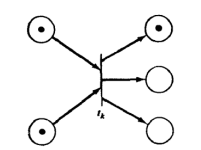
\includegraphics[width=0.3\linewidth]{images/image1.png}}
\caption{Информационная ситуация "одновременность"}
\label{fig1}
\end{figure}

В исходном состоянии имеются два места S, переход обозначен tk отношения инцидентности стрелками. Другая информационная ситуация, в которой одновременное выполнение затруднено и которая характеризуется невозможностью одновременного возникновения событий, показана на рис. \ref{2}. Здесь два разрешенных перехода находятся в конфликте. Может быть запущен только один переход, так как при запуске он удаляет метку из общего входа и запрещает другой переход.

Еще одним достоинством сетей Петри является то, что они моделируются с помощью достаточно простого языка, включающего простые (графические) информационные единицы \cite{Ghanem}. Применение информационных единиц \cite{Tsvetkov3} позволяет использовать лингвистические модели для описания моделей и моделирования на этой основе.

\begin{figure}[ht]
\centerline{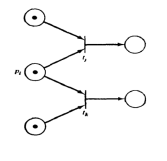
\includegraphics[width=0.3\linewidth]{images/image2.png}}
\caption{Информационная ситуация "Конфликт"}
\label{fig2}
\end{figure}

\section{Моделирование конечных автоматов с применением сетей Петри}

Конечный автомат \cite{Alur} – абстрактный автомат без выходного потока, число возможных состояний которого конечно. Результат работы автомата определяется по его конечному состоянию. Существуют различные варианты задания конечного автомата.

Например, конечный автомат может быть задан с помощью пяти параметров:
\begin{equation}
M = (Q, \Sigma, \delta, q_{0}, F)
\end{equation}
\\где:
\begin{itemize}
  \item $Q$ - конечное множество состояний автомата;
  \item $q_0$ - начальное состояние автомата ($q_0 \in Q$)
  \item $F$ - множество заключительный (или допускающих) состояний, таких, что $F \subseteq Q$
  \item $Sigma$ - допустимый входной алфавит (конечное множество допустимых входных символов), из которого формируются строки, считываемые автоматом
  \item $\delta$ - заданное отображение множества $Q \times \Sigma$ во множество $P(Q)$ подмножеств $Q: \delta : Q \times \Sigma \to P(Q)$ (иногда $\delta$ называют функцией переходов автоматов)
\end{itemize}

Важно отметить, что автоматы часто представляются в виде графов-переходов. Моделирование в рамках сети Петри осуществляется посредством представления алфавитов автомата (входного или выходного) позициями или переходами (рис.\ref{fig3}, рис.\ref{fig4}). Обычно входы представляются позициями. Приведём небольшой пример:

\begin{figure}[ht]
\centerline{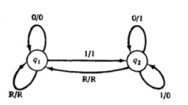
\includegraphics[width=0.3\linewidth]{images/image3.png}}
\caption{Граф конечного автомата, вычисляющего дополнение до двух}
\label{fig3}
\end{figure}

\begin{figure}[ht]
\centerline{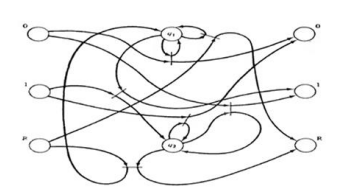
\includegraphics[width=0.3\linewidth]{images/image4.png}}
\caption{Эквивалентная сеть Петри}
\label{fig4}
\end{figure}

Основным применением сетей Петри является возможность преобразования блок-схемы в сеть Петри. Поэтому в виде сети Петри можно представить любой готовый алгоритм, который построен на вычислениях и ветвлениях. \ref{fig5}  иллюстрирует правила перевода. Слева даны классические блок схемы алгоритма, справа - их эквивалент в нотации сети Петри.

\begin{figure}[ht]
\centerline{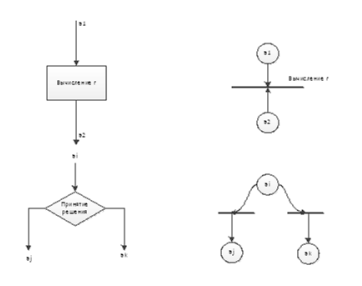
\includegraphics[width=0.5\linewidth]{images/image5.png}}
\caption{Правила перевода блок-схемы в сеть Петри}
\label{fig5}
\end{figure}

\section{Параллельные вычисления и синхронизация}

Сети Петри являются инструментом моделирования процессов и состояний систем \cite{Tsvetkov4}. Большое применение сети Петри нашли при создании и выполнении параллельных ветвей различных вычислительных процессов. На рис. 6 изображена одна из типичных конструкций fork/join. Переход fork моделирует «разветвление» – создание из одной ветви выполнения двух параллельных ветвей. Это, как правило, реализуется путем создания одной дополнительной ветви вдобавок к существующей. Переход join, в свою очередь, осуществляет «слияние» двух ветвей по завершению их работы – уничтожение созданной параллельной ветви за ненадобностью.

\begin{figure}[ht]
\centerline{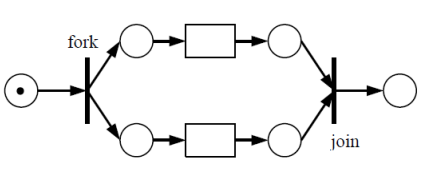
\includegraphics[width=0.5\linewidth]{images/image6.png}}
\caption{Конструкция разветвления-слияния в формализме сети Петри}
\label{fig6}
\end{figure}

Объекты синхронизации также легко моделируются сетями Петри. На рис. \ref{fig7} изображен фрагмент сети Петри, моделирующий барьерную синхронизацию трех процессов.

\begin{figure}[ht]
\centerline{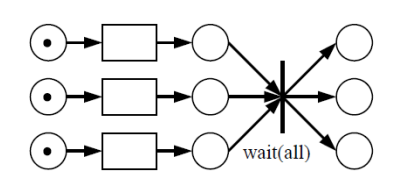
\includegraphics[width=0.5\linewidth]{images/image7.png}}
\caption{Фрагмент сети Петри, моделирующий барьерную синхронизацию
трех процессов}
\label{fig7}
\end{figure}

В начале работы сети разрешенными являются три длительных перехода, характеризующих выполнение некоторых подзадач. Три независимых процесса выполняют эти подзадачи, и лишь после их полного завершения становится разрешенным переход-барьер wait(all). После его срабатывания все три процесса снова продолжают свою работу.

Похожим образом может быть смоделировано ожидание завершения любой из подзадач, первой завершившей свое выполнение. На рис. \ref{fig8} показан такой фрагмент сети. При завершении выполнения любого длительного перехода становится разрешенным переход wait(any). После его срабатывания дальнейшая работа продолжается, в то время как остальные подзадачи завершают свое выполнение. Дополнительная входная позиция перехода wait(any) защищает его от срабатывания при завершении остальных подзадач в случае, если в текущий момент ожидание не выполняется. В процессе дальнейшей работы сети метка в эту позицию возвращается, и тем самым разрешается ожидание и обработка результатов выполнения остальных подзадач.

\begin{figure}[ht]
\centerline{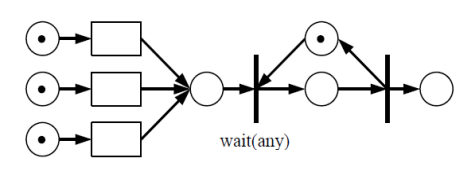
\includegraphics[width=0.5\linewidth]{images/image8.png}}
\caption{Фрагмент сети, моделирующий ожидание завершения любой из подзадач}
\label{fig8}
\end{figure}

Другой пример синхронизации параллельных процессов – критическая секция. Фрагмент сети на рис. \ref{fig9} обеспечивает взаимоисключающий доступ к некоторому общему ресурсу для двух процессов. Первый процесс, захвативший доступ к критической секции, лишит метки соответствующую позицию res, тем самым запретив доступ к критической секции второму процессу до момента ее освобождения. В случае, когда в позиции res изначально более одной метки, такой фрагмент сети моделирует использование семафора – объекта синхронизации, позволяющего одновременный доступ к ресурсу нескольких процессов в количестве не более заданного.

\begin{figure}[ht]
\centerline{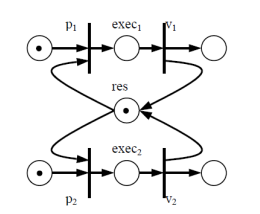
\includegraphics[width=0.5\linewidth]{images/image9.png}}
\caption{Фрагмент сети обеспечивает взаимоисключающий доступ к некоторому общему ресурсу для двух процессов}
\label{fig9}
\end{figure}

Важная особенность сетей Петри заключается в атомарности срабатывания перехода и, как следствие, возможности атомарного захвата одновременно нескольких ресурсов, что исключает взаимоблокировки процессов (dead lock)

Одной из классических задач, иллюстрирующих проблемы синхронизации процессов, является задача об обедающих философах. Ее постановка довольно проста и вкратце заключается в следующем. За круглым столом сидят пятеро философов, перед ними стоит блюдо спагетти. На столе лежат пять вилок - по одной между каждыми двумя соседними философами. По условию каждому философу для еды необходимо две вилки - лежащие непосредственно слева и справа от него. Каждый философ пребывает за столом в одном из двух состояний - размышляет или ест. В последнем случае оба его ближайших соседа размышляют, поскольку для еды им не хватает вилок.

Основная проблема, иллюстрируемая этой задачей - проблема возможности взаимоблокировки, которая была описана раньше. В случае реализации с последовательным захватом вилок возможна ситуация, когда одновременно все философы возьмут, к примеру, левую от себя вилку. Тогда ни один из них не сможет взять правую вилку, и каждый окажется заблокированным в ожидании ее освобождения. На рис. \ref{fig10} изображена сеть Петри, решающая задачу об обедающих философах.

\begin{figure}[ht]
\centerline{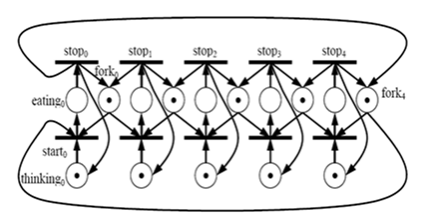
\includegraphics[width=0.5\linewidth]{images/image10.png}}
\caption{Задача об обедающих философах}
\label{fig10}
\end{figure}

Позиции eating и thinking здесь характеризуют пребывание соответствующего философа в состоянии еды или размышлений. Позициями fork обозначается доступность вилок. Переходы start и stop характеризуют переход философа к еде и к размышлениям соответственно. 

Однократный процесс приема пищи каждым философом представляет собой длительную операцию и может быть представлен в виде длительного составного перехода. В этом случае срабатывание перехода stop характеризует завершение приема пищи философом и, соответственно, завершение длительного перехода. Одним из довольно простых решений этой проблемы, хотя, конечно, далеко не самым лучшим, является следующее. К сети, изображенной на рис. \ref{fig11}, добавим барьерную синхронизацию после того, как каждый философ осуществит прием пищи по одному разу.

\begin{figure}[ht]
\centerline{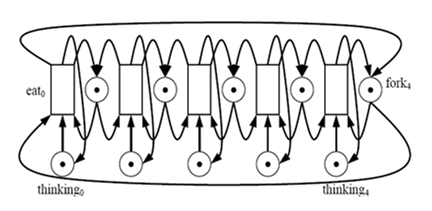
\includegraphics[width=0.5\linewidth]{images/image11.png}}
\caption{Другое представление задачи}
\label{fig11}
\end{figure}

Для этого добавим к каждому философу по две позиции - позицию todo, количество фишек в которой отражает количество предстоящих подходов философа к еде до следующего барьера, и позицию done, отражающую количество выполненных подходов. Полученная сеть изображена на рис. \ref{fig12}

\begin{figure}[ht]
\centerline{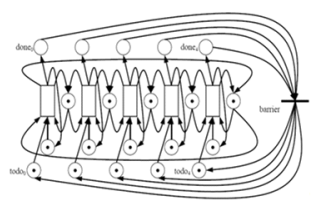
\includegraphics[width=0.5\linewidth]{images/image12.png}}
\caption{Решение задачи вместе с барьером синхронизации}
\label{fig12}
\end{figure}

В случае если синхронизация после каждого подхода к еде является слишком частой мерой, количество фишек в каждой позиции todo может быть увеличено. Более того, начальные количества фишек в этих позициях могут быть заданы разными, в зависимости от потребности в интенсивном питании каждого из философов. В соответствии с начальным количеством фишек в позициях todo должна быть изменена и кратность дуг, ведущих в переход-барьер и из него. 

С учетом такой модификации сети каждый философ будет получать доступ к еде в обычном порядке, пока не закончатся метки в соответствующей позиции todo, после чего остановится на размышлениях. Таким образом, пока каждый из пяти философов не получит доступ к еде заданное количество раз, переход к следующему циклу осуществлен не будет. Когда все метки из позиций todo постепенно переместятся в соответствующие позиции done, переход-барьер снова переместит их в позиции todo, после чего начнется следующий цикл приема пищи. 

\section*{Заключение}

Теория сетей Петри, хотя и возникла как самостоятельная теория \cite{Kotov}, отражает некоторые современные общие тенденции анализа и моделирования. Первая тенденция это применение графических обозначений для формализации процессов и состояний систем. Близким аналогом этому является унифицированный язык визуального моделирования UML \cite{Fowler}. Вторая тенденция это применение информационных единиц как основы информационного языка и основы построения информационных конструкций \cite{Tsvetkov5} и информационных моделей \cite{Breeden}. 

Теория сетей Петри является популярным формализмом, предназначенным для 21 работы с параллельными и асинхронными системами \cite{Leskin}. Она содержит большое количество методов и средств анализа, позволяющих применять ее при моделировании и анализе ряда сложных систем и структурных логических моделей \cite{Tsvetkov6} сложных и информационных систем. Основными особенностями это графической модели является возможность моделирования состояний и переходов между ними. Сеть Петри позволяет проводить анализ процессов за счёт разделения на позиции и переходы. Одна схема может многократно использоваться для описания разных состояний или разных информационных ситуаций. Именно на аспект информационного взаимодействия обращена данная работа. Это поможет в организации информационного моделирования на основе применения сетей Петри.

\begin{thebibliography}

\bibitem{Petri}
Petri, C.
Kommunikation mit Automaten
PhD thesis, University of Bonn, Germany.

\bibitem{Tsvetkov1}
Tsvetkov V. Yа.
Information interaction
European Researcher, 2013, Vol.(62), №11-1 , p.2573- 2577.

\bibitem{Tsvetkov2}
Tsvetkov V. Yа.
Information Situation and Information Position as a Management Tool
European Researcher, 2012, Vol.(36), № 12-1, p.2166- 2170.

\bibitem{Meldman}
Meldman J. A., Holt A. W.
Petri nets and legal systems
Jurimetrics journal. – 1971. – С. 65-75.

\bibitem{Kulagin}
Кулагин В.П., Цветков В.Я. 
Философия сетей Петри
Вестник МГТУ МИРЭА «MSTU MIREA HERALD» 2014 - № 4 (5) - с.18-38.

\bibitem{Peterson}
Peterson J. L. 
Petri nets
Computing Surveys, Vol 9, No. 3, September 1977. - pp.223-252.

\bibitem{Ghanem}
Ghanem N. 
Representation and recognition of events in surveillance video using petri nets 
Computer Vision and Pattern Recognition Workshop, 2004. CVPRW'04. Conference on. – IEEE, 2004. – С. 112-112.

\bibitem{Tsvetkov3}
Tsvetkov V. Ya.
Information Units as the Elements of Complex Models
Nanotechnology Research and Practice, 2014, Vol.(1), № 1. р57-64.

\bibitem{Ozhereleva}
Ozhereleva T. А. 
Systematics for information units
European Researcher, 2014, Vol.(86), № 11/1, pp. 1894-1900.

\bibitem{Alur}
Alur R., Dill D. L. 
A theory of timed automata
Theoretical computer science. – 1994. – V. 126. , №. 2. –pp.183-235.

\bibitem{Tsvetkov4}
Цветков В.Я. 
Моделирование в автоматизации научных исследований и проектировании.
ВНТИЦентр, 1991. – 125с.

\bibitem{Kotov}
Котов В.Е.
Сети Петри
М.:Наука, 1984.-160с.

\bibitem{Fowler}
Fowler M. 
UML distilled: a brief guide to the standard object modeling language.
Addison-Wesley Professional, 2004.

\bibitem{Tsvetkov5}
Tsvetkov V. Ya. 
Information Constructions
European Journal of Technology and Design, 2014, Vol.(5), № 3- p147-152.

\bibitem{Breeden}
Breeden D., Viswanathan S. 
Why do firms hedge? An asymmetric information model
Fuqua School of Business, Working Paper. – 1998.

\bibitem{Leskin}
А.А. Лескин, П.А. Мальцев, А.М. Спиридонов
Сети Петри в моделировании и управлении
Наука, 1989.-133с.

\bibitem{Tsvetkov6}
Tsvetkov V.Ya. 
Logic units of information systems
European Journal of Natural History. - 2009. - № 2 . - p 99-100.

\end{thebibliography}

\end{document}
